\documentclass[aspectratio=169,xcolor=dvipsnames]{beamer}
\usepackage{tikz}
\usepackage{graphicx}
\usepackage{parskip}
\usepackage[absolute,overlay]{textpos}
\usepackage{amsmath}
\usepackage{booktabs}
\usetikzlibrary{shapes.geometric, arrows.meta, positioning, calc}
\usetheme{CambridgeUS}

\definecolor{IITHorange}{RGB}{243, 130, 33}
\definecolor{IITHyellow}{RGB}{254, 203, 10}

\setbeamercolor{palette primary}{bg=IITHorange,fg=white}
\setbeamercolor{palette secondary}{bg=IITHorange,fg=white}
\setbeamercolor{palette tertiary}{bg=IITHorange,fg=white}
\setbeamercolor{palette quaternary}{bg=IITHorange,fg=white}
\setbeamercolor{structure}{fg=IITHorange}
\setbeamercolor{section in toc}{fg=IITHorange}
\setbeamercolor{subsection in head/foot}{bg=IITHyellow,fg=white}

\title[]{Physically-Motivated Compound-Degradation Image Restoration}
\subtitle{KLA AI Hackathon, IITH'26}
\date{\today}
\author[]
{Supriyo Banerjea (AI24MTECH12005)\\Debanjan Das (AI24MTECH12009)\\Sumanta Manna (AI24MTECH12011)}
\institute[]{Department of Artificial Intelligence\\ \textbf{Indian Institute of Technology, Hyderabad}}

\begin{document}
	
	\begin{frame}
		\titlepage
        % \begin{textblock*}{1.5cm}(11.5cm,7.7cm)
        %   
\includegraphics[width=1cm]{images/Screenshot 2025-12-30 091729.png}
        % \end{textblock*}
	\end{frame}
	
	\begin{frame}
    \frametitle{Outline}
		\tableofcontents
	\end{frame}
	
	\section{Problem Statement \& Dataset Overview}
	\begin{frame}
        \frametitle{Problem Statement \& Dataset Overview}
        \begin{itemize}
            \item \textbf{Objective:} Develop a robust model to reconstruct high-quality images from degraded, noisy, low-resolution (\texttt{.npy}) inputs.
            \item \textbf{Challenge:} Real-world physical degradation is complex, requiring models to handle \textbf{compound corruptions} simultaneously (Speckle + AWGN + Downsampling).
            \item \textbf{Dataset:} Supervised pairs of degraded $\leftrightarrow$ Ground Truth ($256\times256$). Test set includes out-of-distribution samples to evaluate generalization.
            \item \textbf{Evaluation:} Joint optimization of \texttt{MSE, PSNR, SSIM, LPIPS} + Inference speed.
        \end{itemize}
        % \vspace{0.5em}
        \begin{center}
            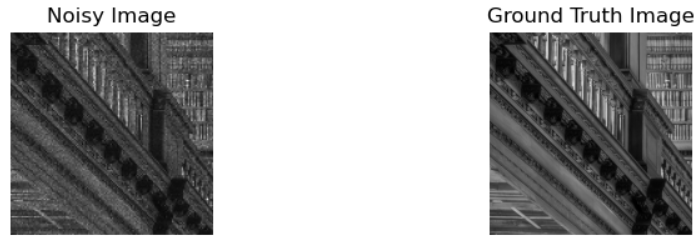
\includegraphics[width=0.45\textwidth]{images/noisy_gt_comp.png}
            % \captionof{figure}{\footnotesize Sample degraded vs. Ground Truth pair}
        \end{center}
    \end{frame}

\section{EDA Insights}
% \begin{frame}{Exploratory Data Analysis (EDA) Insights}
%     \framesubtitle{Statistical Modeling of Noise Distributions}
%     \begin{itemize}
%         \item \textbf{Residual Analysis:} Analyzed the pixel-wise differences between NoisyLR and Ground Truth samples.
%         \item \textbf{Distribution Fitting:} Evaluated statistical fits for the noise profile using Negative Log-Likelihood (NLL) and Akaike Information Criterion (AICC).
%         \item \textbf{Key Findings:} Compared \textbf{Gaussian} vs. \textbf{Student-t} distributions to model the heavy-tailed nature of the noise, revealing that standard Gaussian assumptions fail to capture structural outliers and extreme artifacts.
%     \end{itemize}
%     \vspace{0.4cm}
%     % \begin{center}
%     %     % \includegraphics[width=0.5\textwidth]{distribution_plot.png}
%     %     \textit{[Insert Image: Gaussian vs Student-t distribution plot]}
%     % \end{center}
% \end{frame}

\begin{frame}{Motivation behind EDA}
  \begin{itemize}
    \item \textbf{Objective:} Statistically predict the image degradation process to understand its effect on the possible manifold space, serving as an additional supervision prior for the restoration task.
    \item \textbf{Context:} We do not know the exact noise distribution of the images used during the NAFNet pretraining phase.
    \item \textbf{Hypothesis:} By embedding the physical behavior of our specific case (Down-sampling + Speckle + AWGN) into the finetuning process, the model's performance can be significantly improved.
    \item \textbf{Role of EDA:} Rather than perfectly estimating deterministic parameters, EDA helps us identify the most likely random perturbations from possible options and estimate their underlying parameter ranges.
  \end{itemize}
\end{frame}

\begin{frame}{Spatial Match \& Proxy Downsampling}
  \begin{columns}
    \begin{column}{0.6\textwidth}
      \begin{itemize}
        \item \textbf{Scale Factor:} The noisy images are downsampled by a factor of $2 \times 2$ compared to the ground truth.
        \item \textbf{Proxy Downsampling:} Evaluated Nearest Neighbor vs. Block Mean.
        \item \textbf{Selection:} The \texttt{block\_mean} approach is the optimal proxy due to a significantly lower residual MSE ($0.0081$ vs $0.0104$).
      \end{itemize}
    \end{column}
    \begin{column}{0.4\textwidth}
      \begin{figure}
        % Replace with the actual filename of your downsampling plot from the notebook
        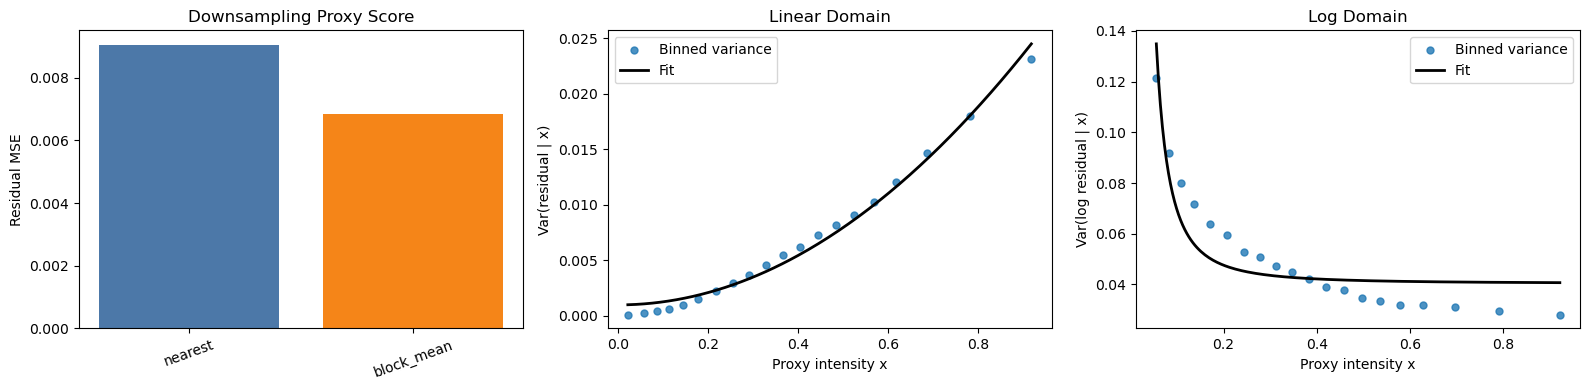
\includegraphics[width=\linewidth]{images/downsample.png} 
        \caption{Downsampling Proxy Comparison}
      \end{figure}
    \end{column}
  \end{columns}
\end{frame}

\begin{frame}{Noise Modeling: Speckle \& Additive}
  \begin{columns}
    \begin{column}{0.5\textwidth}
      \begin{itemize}
        \item \textbf{Linear Model:} $Var(r|x) \approx a \cdot x^2 + b$
        \begin{itemize}
            \item Speckle noise ($\sigma \approx 0.167$)
            \item Additive noise ($\sigma \approx 0.031$)
        \end{itemize}
        \item \textbf{Log-Domain \& PCA:} Log residual analysis reveals a significant $1/x^2$ term. PCA on linear residuals cross-checks a baseline variance ($\sigma \approx 0.021$).
        \item \textbf{Implication:} The noise is a complex mix of multiplicative and additive components.
      \end{itemize}
    \end{column}
    \begin{column}{0.5\textwidth}
      \begin{figure}
        % Replace with the actual filename of your variance/noise fit plot from the notebook
        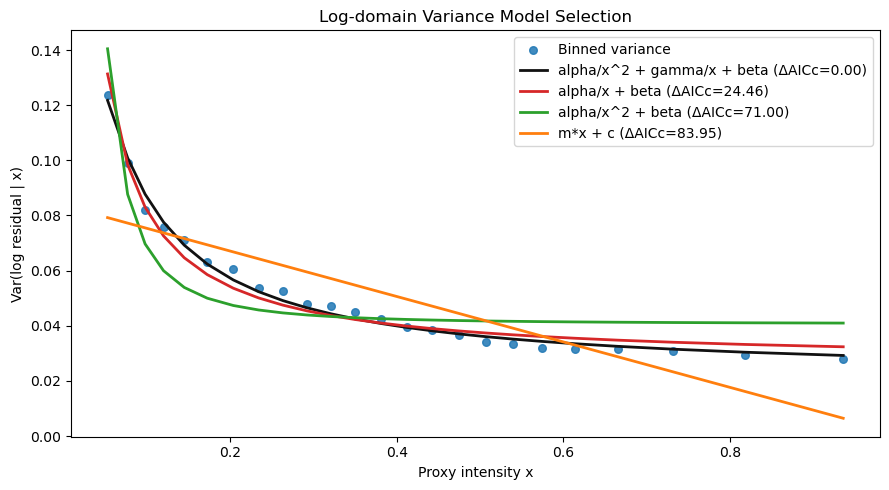
\includegraphics[width=\linewidth]{images/noise_variance.png}
        \caption{Noise Variance Model Fit}
      \end{figure}
    \end{column}
  \end{columns}
\end{frame}

\begin{frame}{Degradation Pipeline Hypothesis}
  \begin{itemize}
    \item \textbf{Goal:} Determine the chronological sequence of degradation.
    \item \textbf{Hypotheses Tested:}
    \begin{itemize}
        \item \textbf{H1:} Downsample $\rightarrow$ Speckle $\rightarrow$ Additive
        \item \textbf{H2:} Speckle $\rightarrow$ Downsample $\rightarrow$ Additive
    \end{itemize}
    \item \textbf{Results:} AICc ranking strongly favors \textbf{H2} ($\Delta AICc = 0.00$). H1 incurs a heavy statistical penalty.
  \end{itemize}
  
  \vspace{0.5cm}
  \begin{center}
    \textbf{Final Inferred Pipeline:}\\
    \textit{Ground Truth $\rightarrow$ Speckle Noise $\rightarrow$ Block Mean Downsample $\rightarrow$ AWGN}
  \end{center}
 \end{frame}
 \begin{frame}{Hypothesis Comparison}
  \begin{figure}
    % Replace with a relevant plot (e.g. AICc comparison or residuals) from the notebook, or remove if not needed
    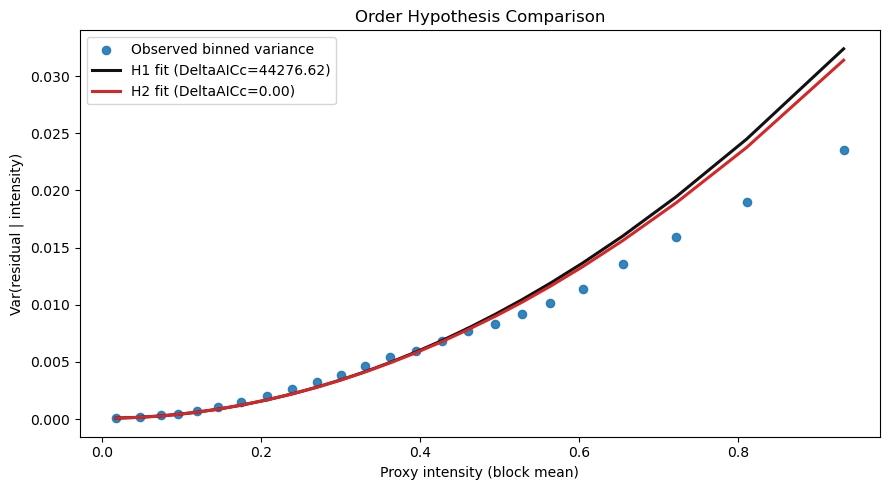
\includegraphics[height=7cm]{images/hypothesis_comparison.png}
  \end{figure}
\end{frame}

    \section{Proposed Architecture: NAFNetH2SR}
    
    \begin{frame}
        \frametitle{NAFNet: Nonlinear Activation Free Network}
        \begin{itemize}
            \item \textbf{Architecture:} Single-stage U-Net with dense skip connections (low inter-block complexity).
            \item \textbf{Critical Innovation:} Removes standard nonlinear activations (ReLU, GELU, Sigmoid) entirely.
            \begin{itemize}
                \item \textbf{SimpleGate:} Replaces GELU with element-wise multiplication of channel-split features: 
                \[ Y = X_1 \odot X_2 \]
                Nonlinearity is introduced purely via gating, mimicking GLU without extra activations.
                \item \textbf{Simplified Channel Attention (SCA):} Removes ReLU/Sigmoid from CA. Uses global average pooling and a linear projection to reweight channels efficiently.
            \end{itemize}
            \item \textbf{Result:} A ``nonlinear activation-free'' network that simplifies the computational graph, stabilizes training, and drastically reduces MACs.
        \end{itemize}
    \end{frame}

    \begin{frame}
        \frametitle{Why NAFNet Revolutionized Efficient Image Restoration}
        \begin{columns}[T]
            \begin{column}{0.5\textwidth}
                \begin{itemize}
                    \item \textbf{State-of-the-Art Performance:} Achieves $\sim 40.30$ dB PSNR on SIDD and $\sim 33.69$ dB on GoPro benchmarks.
                    \item \textbf{Computational Efficiency:} 
                    \begin{itemize}
                        \item $<50\%$ MACs of Restormer (Denoising).
                        \item Only $8.4\%$ MACs of MPRNet (Deblurring).
                    \end{itemize}
                    \item \textbf{Why it works:} Replaces expensive self-attention maps and multi-stage pipelines with simple convolutions + element-wise gates.
                    \item \textbf{Hackathon Fit:} High efficiency enables rapid inference optimization and fits within strict compute constraints while maximizing SSIM/LPIPS.
                \end{itemize}
            \end{column}
            \begin{column}{0.5\textwidth}
                \centering
                \vspace{0.5em}
                \textbf{PSNR vs. MACs (SIDD Benchmark)}
                \vspace{0.5em}
                % Replace with actual plot if available
                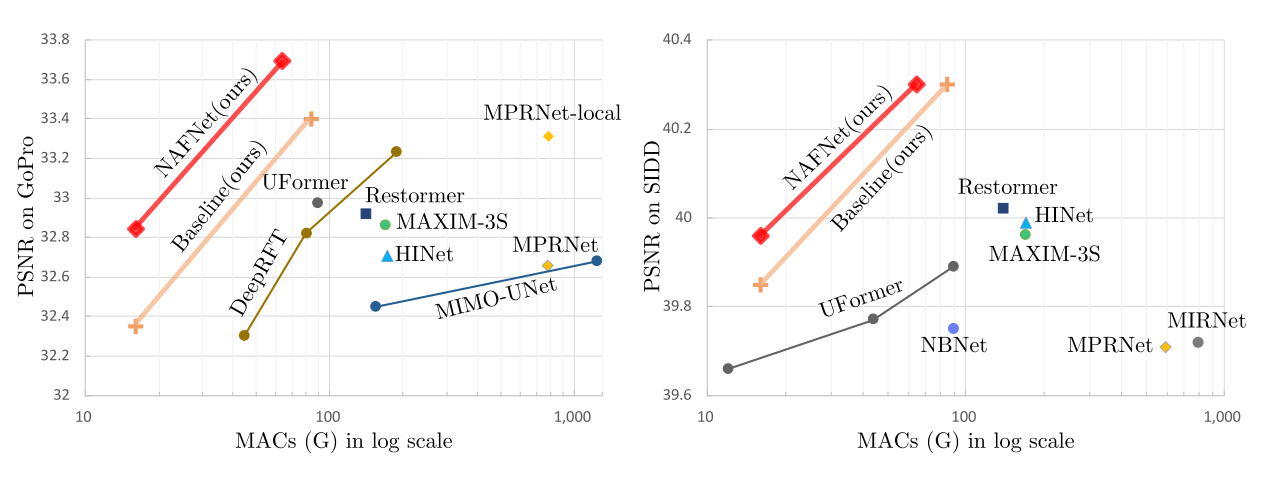
\includegraphics[height=3cm]{macs-psnr.png}
                % \footnotesize \textit{``SOTA achieved by a simple baseline without nonlinear activation functions.''}
            \end{column}
        \end{columns}
    \end{frame}

    \begin{frame}
        \frametitle{Our Implementation: \texttt{NAFNetH2SR} for Joint SR \& Denoising}
        \textbf{Adapting NAFNet to our Compound Degradation Challenge:}
        \begin{itemize}
            \item \textbf{Task:} Joint Speckle/AWGN Denoising + Deblurring + $2\times$ Super-Resolution.
            \item \textbf{Grayscale Handling Pipeline:} 
            \begin{enumerate}
                \item Upsample LR input ($1\times H\times W$) via bicubic interpolation.
                \item \textbf{Replicate to 3 channels} for compatibility with official RGB NAFNet backbone.
                \item Restore via NAFNet $\rightarrow$ \textbf{Collapse to grayscale} via channel-wise mean: $\hat{y} = \frac{1}{3}\sum_{c=1}^3 \hat{x}_c$.
            \end{enumerate}
            \item \textbf{Advantages for Hackathon:}
            \begin{itemize}
                \item \textbf{Robustness:} U-Net structure captures fine-grained noise removal while preserving structural coherence (SSIM/LPIPS friendly).
                \item \textbf{Inference Speed:} Lightweight blocks enable fast processing of large test batches.
                \item \textbf{Output:} Direct $256 \times 256$ float32 grayscale predictions ready for \texttt{.npy} submission.
            \end{itemize}
        \end{itemize}
    \end{frame}
\begin{frame}
        \frametitle{Objective Formulation: Multi-Faceted Loss}
        \begin{columns}[T]
            \begin{column}{0.7\textwidth}
                To prevent over-smoothing and enforce structural fidelity, we employ a dynamically weighted loss landscape:
                \begin{itemize}
                    \item \textbf{Reconstruction (Pixel):} Official NAFNet PSNR Loss (log-scaled MSE) + Charbonnier Loss ($\sqrt{(x-\hat{x})^2 + \epsilon^2}$) for outlier robustness.
                    \item \textbf{Perceptual \& Structural:}
                    \begin{itemize}
                        \item \textbf{SSIM Loss:} Enforces local structural similarity.
                        \item \textbf{LPIPS:} Learned perceptual feature matching.
                    \end{itemize}
                    \item \textbf{Heteroscedastic Data Consistency (DC):}
                    $$\mathcal{L}_{DC} = \frac{1}{N} \sum \log\left(1 + \frac{(y - \mu)^2}{\nu \cdot v}\right)$$
                    A heavy-tailed Student-t formulation bridging the LR input ($y$) and downsampled prediction ($\mu$), isolated from variance collapse.
                \end{itemize}
            \end{column}
            \begin{column}{0.3\textwidth}
                \vspace{1em}
                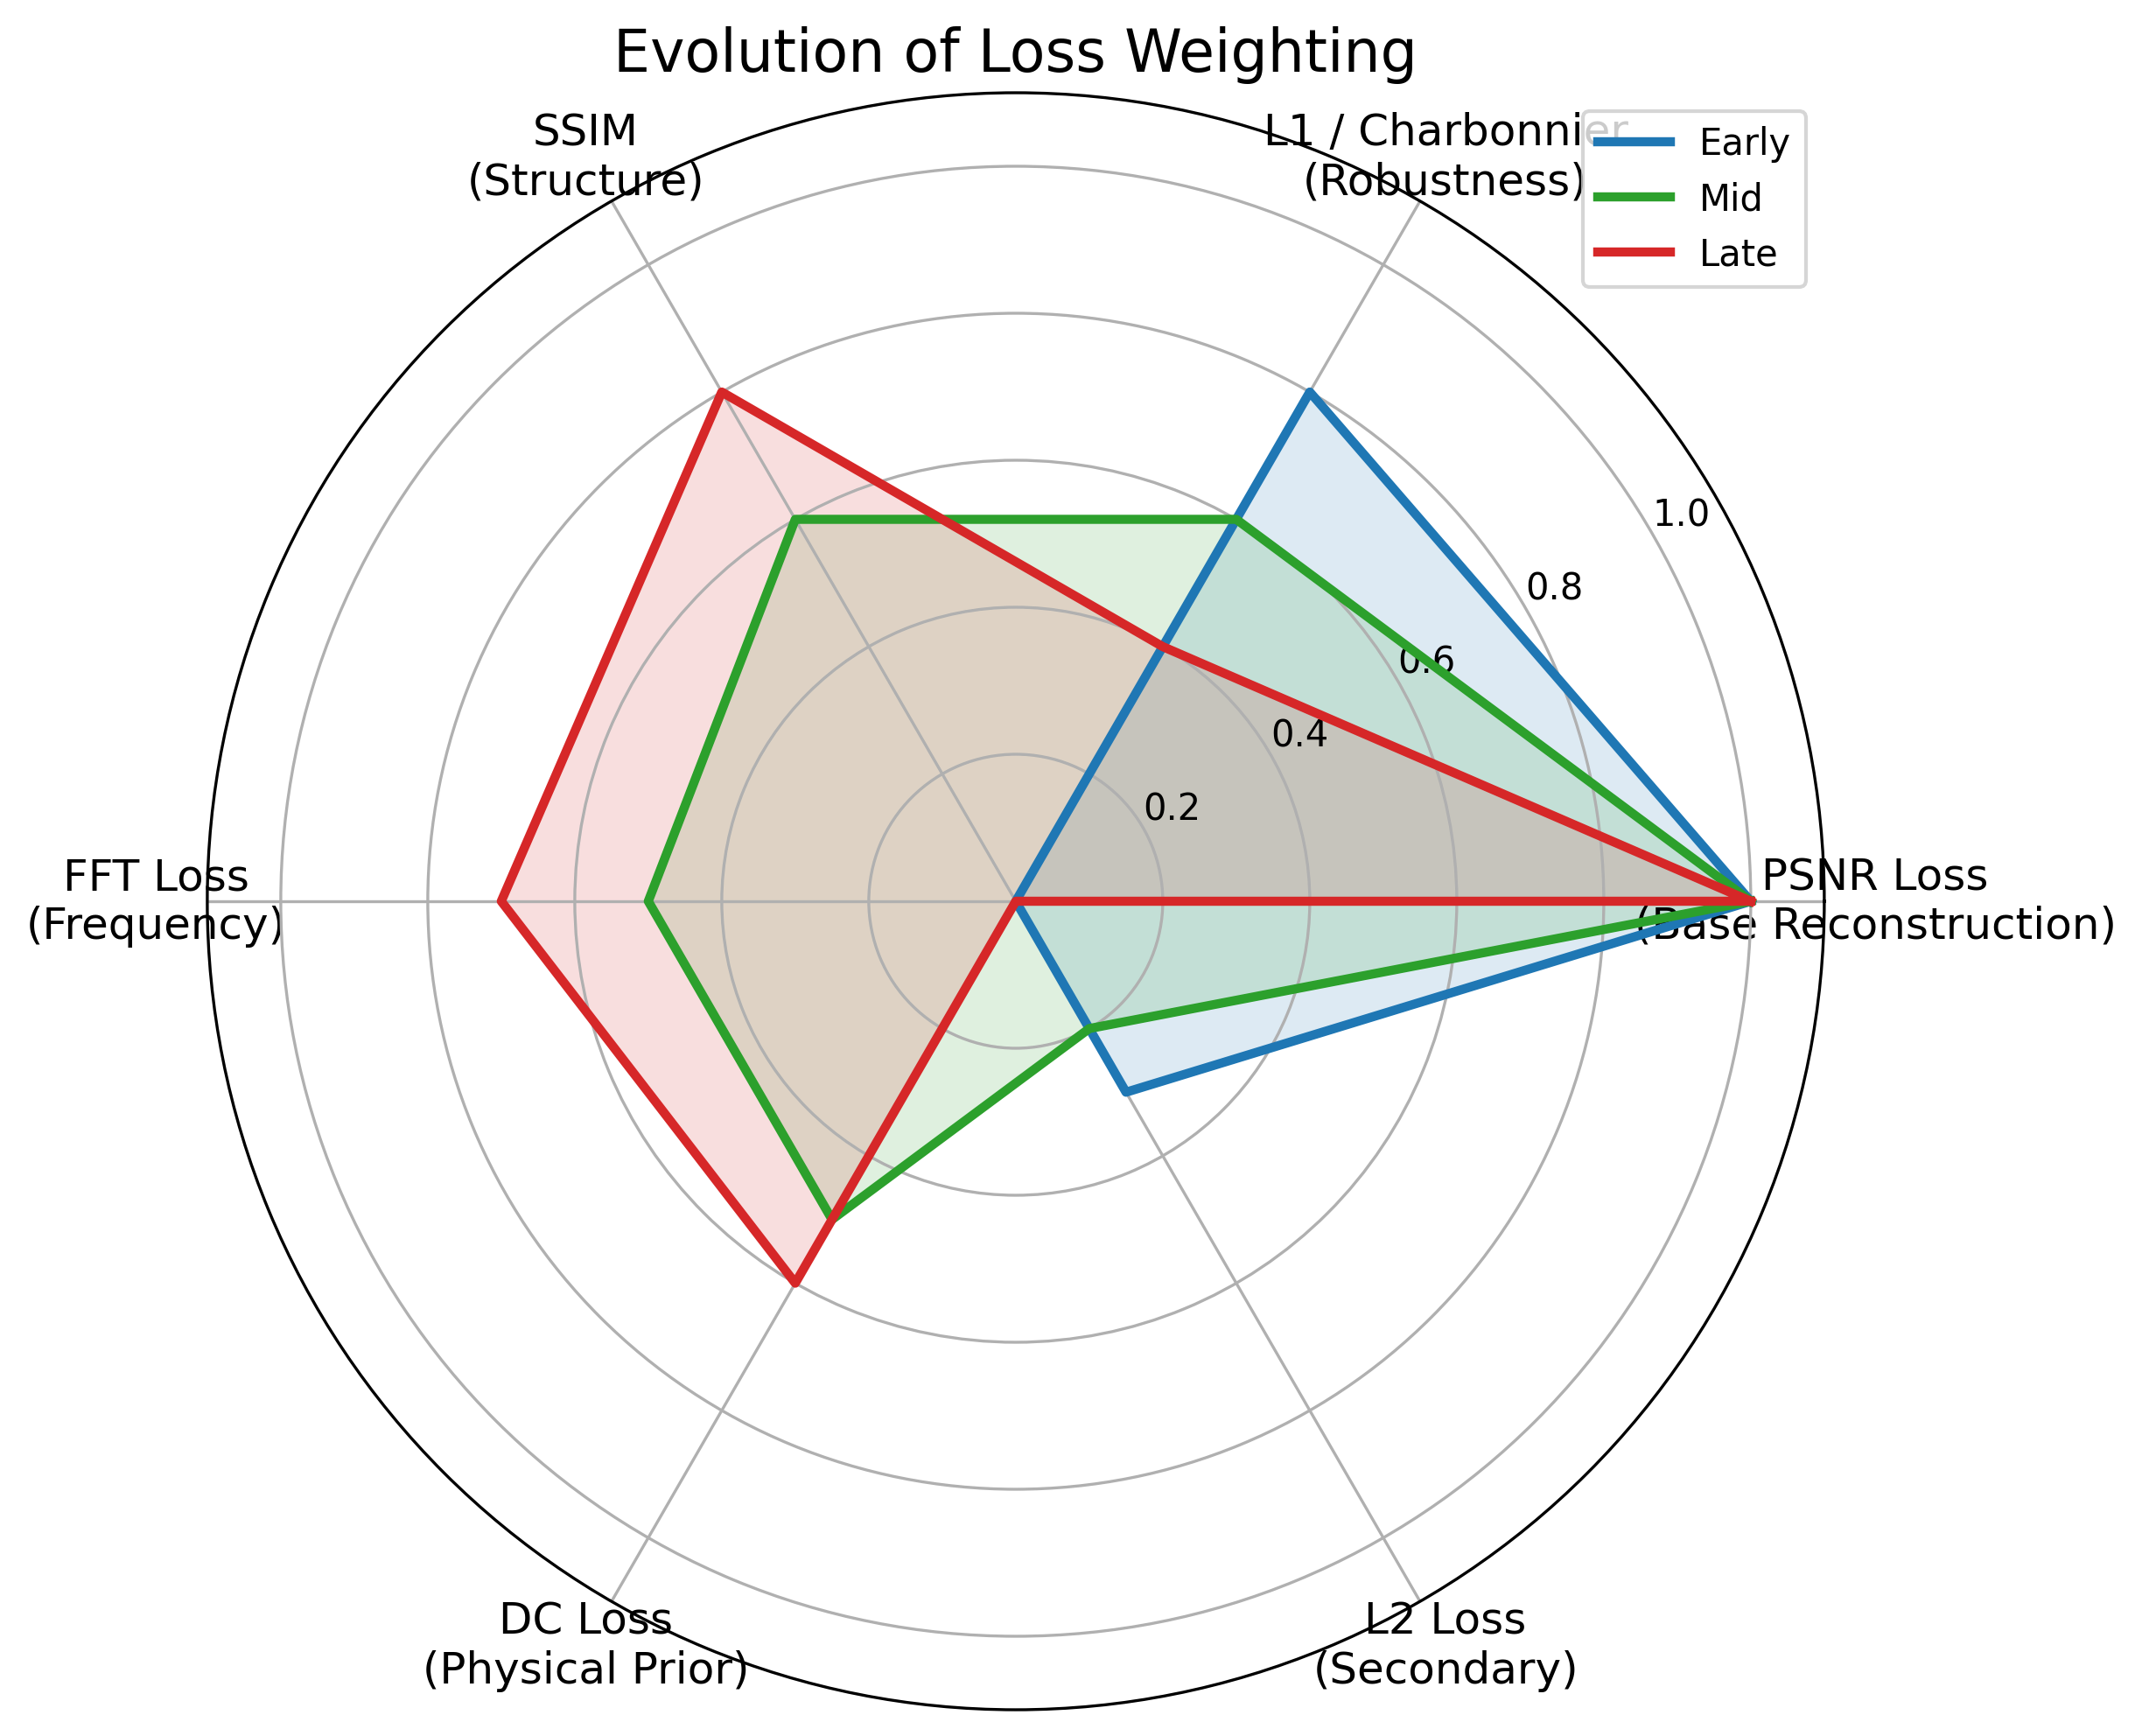
\includegraphics[height=3.5cm]{images/nafnet_loss_radar.png}
                \caption{Weight of the different loss components}
            \end{column}
        \end{columns}
    \end{frame}

\begin{frame}
        \frametitle{Training Dynamics: OOD Augmentation \& Curriculum}
        \textbf{Goal:} Force the network to learn robust feature extraction rather than memorizing the exact noise distribution.
        \begin{itemize}
            \item \textbf{Synthetic OOD Degradations:}
            \begin{itemize}
                \item \textit{Photometric:} Affine shifts, dynamic Gamma correction.
                \item \textit{Noise:} Speckle, Poisson, Gaussian combinations.
                \item \textit{Structural Defects:} 3x3 reflection blur, impulse noise, and spatial cutouts simulating sensor failure.
            \end{itemize}
            \item \textbf{Curriculum Learning Schedule:}
            \begin{itemize}
                \item \textbf{Phase 1 (Robustness):} High probability ($p=0.95$) and max transforms ($n=5$). Early layers frozen to protect pre-trained features.
                \item \textbf{Phase 2 (Finetuning):} Transform probability and intensity linearly decay.
                \item \textbf{Phase 3 (Convergence):} Network fully un-frozen, evaluated primarily on pure dataset distribution.
            \end{itemize}
        \end{itemize}
        % \vspace{0.5em}
        % \fbox{\parbox{\linewidth}{\centering \vspace{1em} \textit{[Diagram Placeholder: \\ 3x3 Grid showing Base Image vs. Synthetic Degradation profiles]} \vspace{1em}}}
    \end{frame}

    \begin{frame}
        \frametitle{Inference Optimization: Maximizing the Test Score}
        \begin{columns}[T]
            \begin{column}{0.5\textwidth}
                \begin{itemize}
                    \item \textbf{Test-Time Augmentation (TTA):} 
                    \begin{itemize}
                        \item \textit{Balanced mode:} 4-way flips.
                        \item \textit{High mode:} 8-way (flips + rotations).
                        \item Averages predictions across spatial transformations to reduce variance.
                    \end{itemize}
                    \item \textbf{Test-Time Refinement:}
                    \begin{itemize}
                        \item Instantiates a local Adam optimizer at inference.
                        \item Performs $N$ gradient steps directly on the predicted HR output to minimize the Data Consistency (DC) loss against the specific test LR image.
                        \item \textit{Result:} Physically "locks in" the prediction to the exact noise profile of the test sample.
                    \end{itemize}
                \end{itemize}
            \end{column}
            \begin{column}{0.5\textwidth}
                \begin{figure}[h]
    \centering
    \resizebox{0.85\linewidth}{!}{% Scale to fit the slide perfectly
    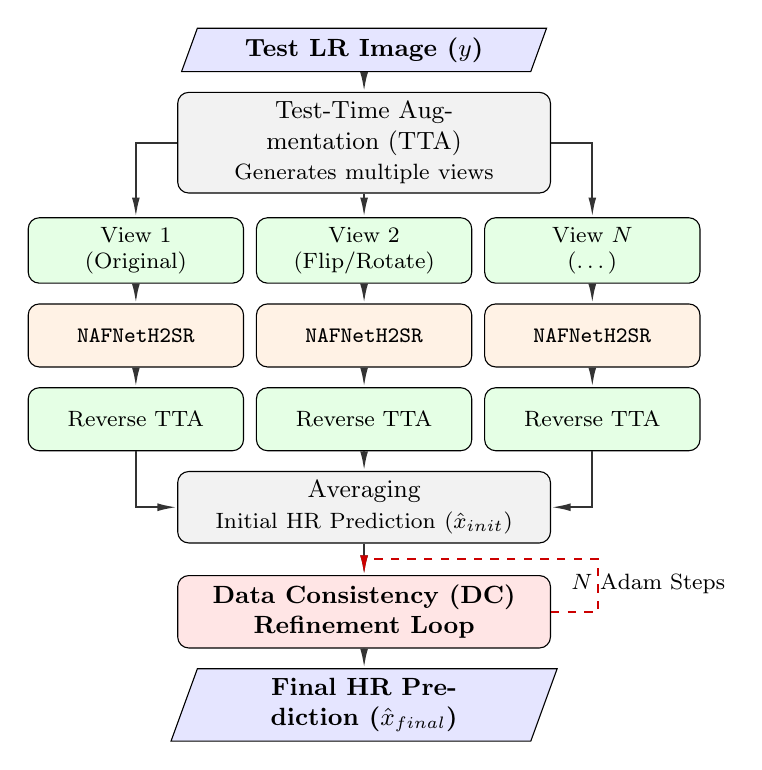
\begin{tikzpicture}[
        node distance=0.4cm and 0.2cm,
        auto,
        % Define styles for the different blocks
        io/.style={trapezium, trapezium left angle=70, trapezium right angle=110, draw, fill=blue!10, text width=4cm, text centered, minimum height=0.4cm, font=\small\bfseries},
        block/.style={rectangle, draw, fill=gray!10, text width=4.5cm, text centered, rounded corners, minimum height=0.4cm, font=\small},
        branch/.style={rectangle, draw, fill=green!10, text width=2.5cm, text centered, rounded corners, minimum height=0.8cm, font=\footnotesize},
        model/.style={rectangle, draw, fill=orange!10, text width=2.5cm, text centered, rounded corners, minimum height=0.8cm, font=\footnotesize\ttfamily},
        refine/.style={rectangle, draw, fill=red!10, text width=4.5cm, text centered, rounded corners, minimum height=0.5cm, font=\small\bfseries},
        line/.style={draw, -{Latex[length=2.5mm, width=1.0mm]}, thick, color=black!80}
    ]

    % --- Nodes ---
    % Input
    \node [io] (input) {Test LR Image ($y$)};
    
    % TTA Split
    \node [block, below=0.25cm of input] (tta) {Test-Time Augmentation (TTA) \\ \footnotesize Generates multiple views};
    
    % Parallel Branches (Views)
    \node [branch, below=0.3cm of tta] (view2) {View 2 \\ (Flip/Rotate)};
    \node [branch, left=0.15cm of view2] (view1) {View 1 \\ (Original)};
    \node [branch, right=0.15cm of view2] (viewN) {View $N$ \\ ($\dots$)};
    
    % Forward Pass (Models)
    \node [model, below=0.25cm of view1] (mod1) {NAFNetH2SR};
    \node [model, below=0.25cm of view2] (mod2) {NAFNetH2SR};
    \node [model, below=0.25cm of viewN] (modN) {NAFNetH2SR};
    
    % Reverse TTA
    \node [branch, below=0.25cm of mod1] (rev1) {Reverse TTA};
    \node [branch, below=0.25cm of mod2] (rev2) {Reverse TTA};
    \node [branch, below=0.25cm of modN] (revN) {Reverse TTA};
    
    % Averaging
    \node [block, below=0.25cm of rev2] (avg) {Averaging \\ \footnotesize Initial HR Prediction ($\hat{x}_{init}$)};
    
    % DC Refinement Loop
    \node [refine, below=0.4cm of avg] (refine) {Data Consistency (DC) \\ Refinement Loop};
    
    % Output
    \node [io, below=0.25cm of refine] (output) {Final HR Prediction ($\hat{x}_{final}$)};

    % --- Edges (Arrows) ---
    \path [line] (input) -- (tta);
    
    % Splitting paths
    \path [line] (tta) -| (view1);
    \path [line] (tta) -- (view2);
    \path [line] (tta) -| (viewN);
    
    % Straight paths down the branches
    \path [line] (view1) -- (mod1);
    \path [line] (view2) -- (mod2);
    \path [line] (viewN) -- (modN);
    
    \path [line] (mod1) -- (rev1);
    \path [line] (mod2) -- (rev2);
    \path [line] (modN) -- (revN);
    
    % Merging paths back to average
    \path [line] (rev1) |- (avg);
    \path [line] (rev2) -- (avg);
    \path [line] (revN) |- (avg);
    
    \path [line] (avg) -- (refine);
    \path [line] (refine) -- (output);
    
    % Refinement Loop Arrow
    \draw [line, dashed, color=red!80!black] 
        (refine.east) -- ++(0.6,0) 
        |- ($ (avg.south) !0.5! (refine.north) $) 
        -| (refine.north) 
        node[pos=1.3, right=2.5cm, font=\footnotesize, text=black] {$N$ Adam Steps};

    \end{tikzpicture}
    }
\end{figure}
            \end{column}
        \end{columns}
    \end{frame}

\section{Results \& Conclusion}

    \begin{frame}
        \frametitle{Quantitative Results \& Leaderboard Performance}
        \begin{columns}[T]
            \begin{column}{0.55\textwidth}
                \textbf{Local Validation (2\% Held-Out):}
                \begin{itemize}
                    \item \textbf{PSNR:} $28.5$ dB
                    \item \textbf{SSIM:} $0.77$
                \end{itemize}
                
                \vspace{1em}
                \textbf{Kaggle Competition Results:}
                \begin{table}[]
                    \centering
                    \renewcommand{\arraystretch}{1.3}
                    \begin{tabular}{l | c c}
                        \textbf{Phase} & \textbf{Score} & \textbf{Rank} \\
                        \hline
                        Public LB & $0.88614$ & $12$ \\
                        \textbf{Private LB} & \textbf{0.88303} & \textbf{10} \\
                    \end{tabular}
                \end{table}
            \end{column}
            \begin{column}{0.45\textwidth}
                \vspace{1em}
                \begin{block}{OOD Generalization Hypothesis}
                    Our model maintained high stability and actually \textbf{climbed two ranks} on the Private Leaderboard. 
                    
                    \vspace{0.5em}
                    We hypothesize this resilience is directly attributable to our \textbf{heavy, curriculum-based OOD data augmentations}. By simulating extreme structural defects and photometric shifts during training, the model generalized perfectly to the unseen, severe degradations in the private test set.
                \end{block}
            \end{column}
        \end{columns}
    \end{frame}

    \begin{frame}{Denoised Images (Randomly Sampled from Noisy Test Set)}
    \centering
        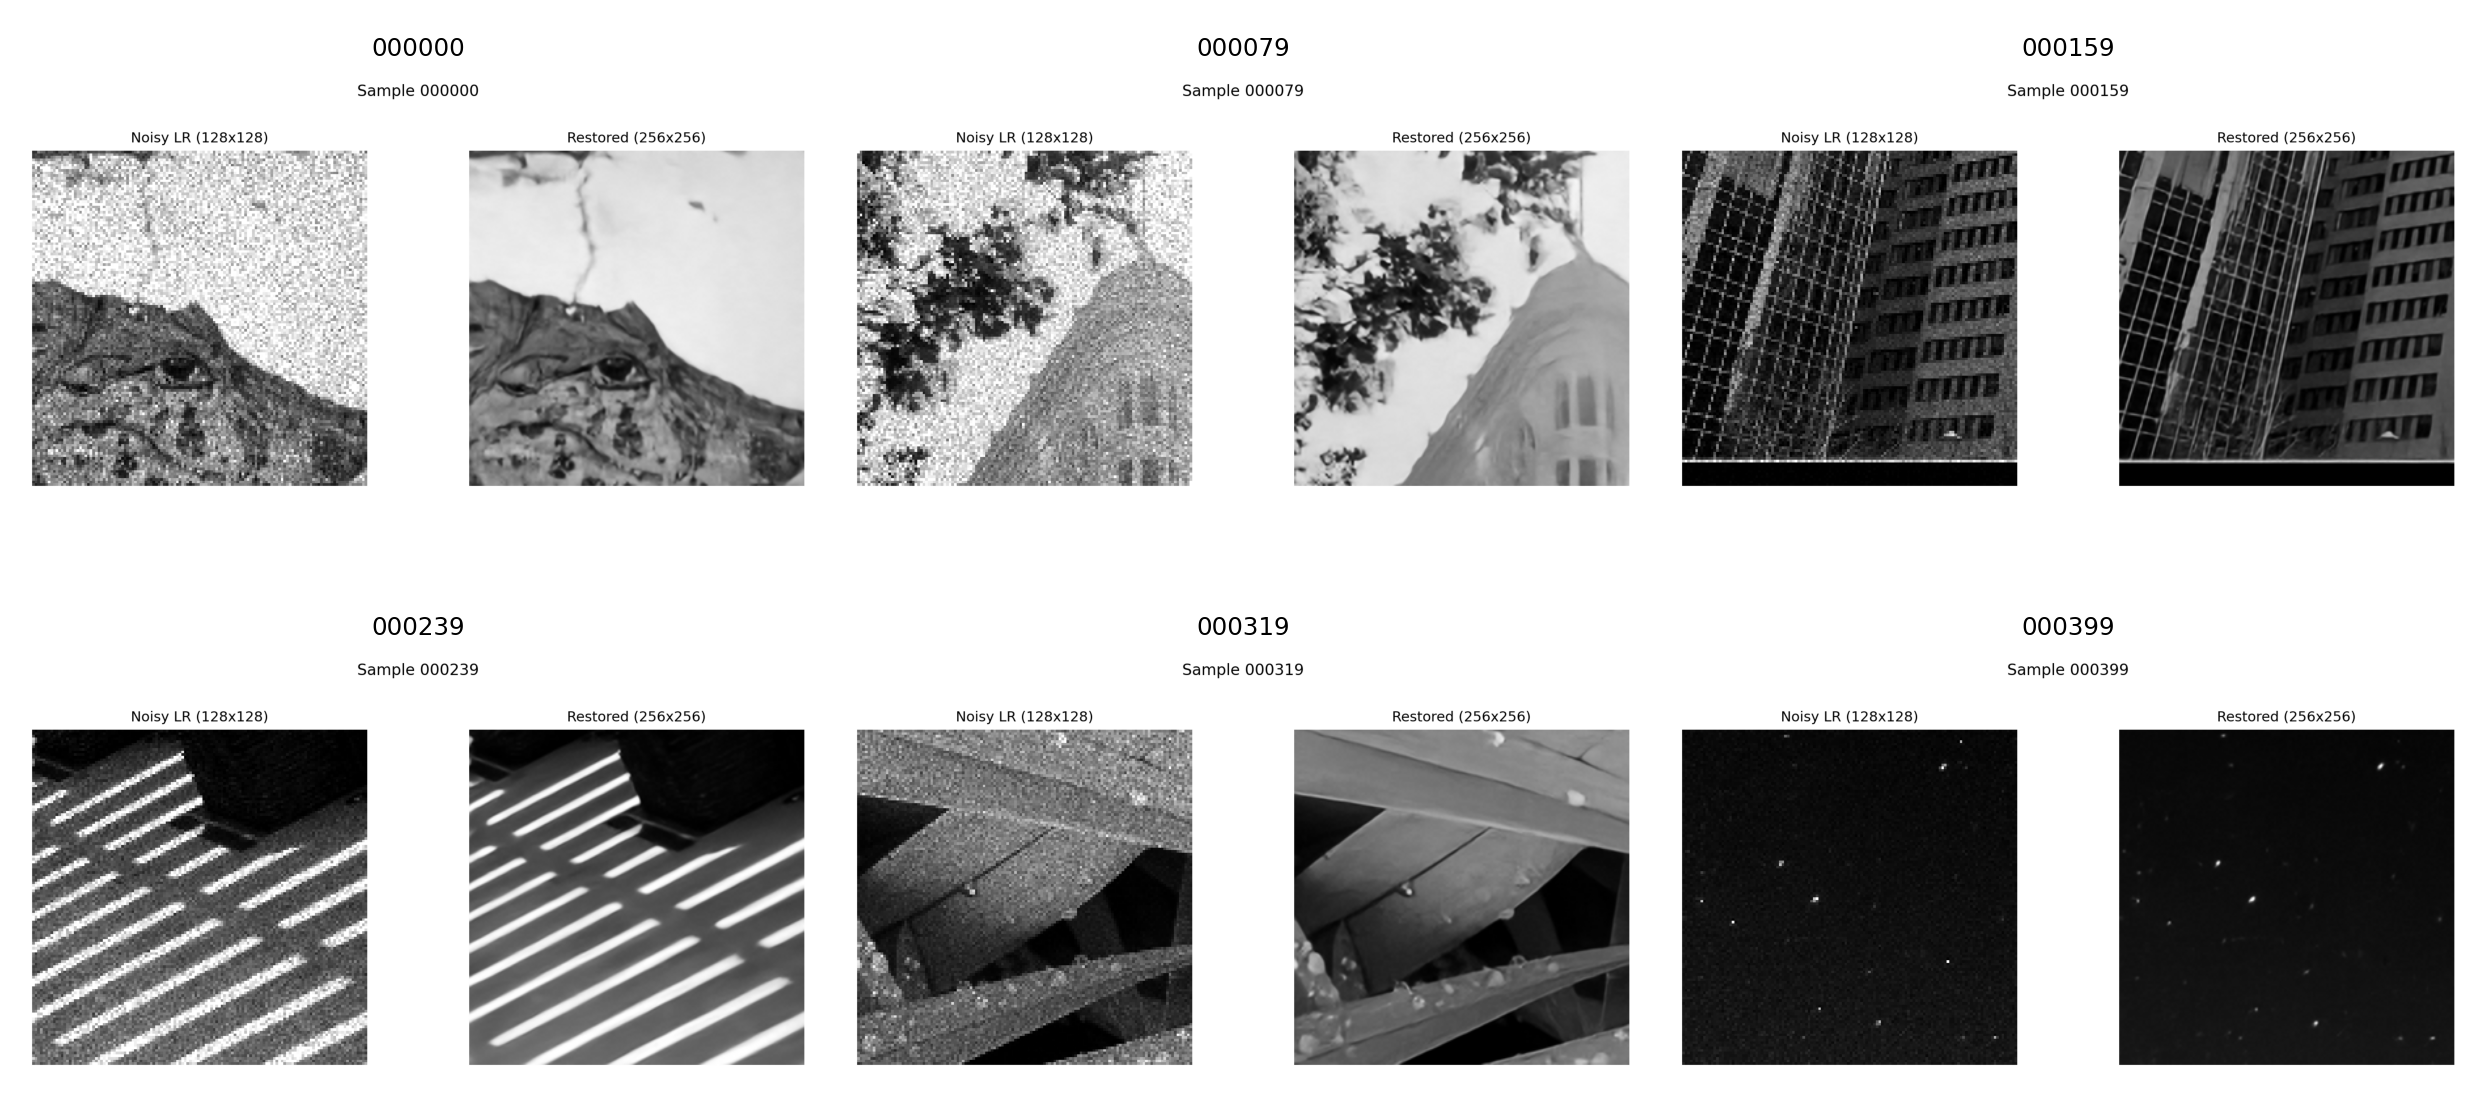
\includegraphics[height=6.75cm]{contact_sheet_6_samples.png}
    \end{frame}
    
    \begin{frame}
        \frametitle{Computational Cost \& Efficiency}
        \textbf{Training Infrastructure \& Constraints:}
        \begin{itemize}
            \item \textbf{Hardware:} $4 \times$ NVIDIA RTX A5000 GPUs.
            \item \textbf{Framework:} PyTorch Distributed Data Parallel (DDP) utilizing Automatic Mixed Precision (AMP).
        \end{itemize}
        
        \vspace{1em}
        \textbf{Performance Metrics:}
        \begin{itemize}
            \item \textbf{Training Time:} $\sim 75$ minutes for a full $120$-epoch run.
            \item \textbf{Efficiency Gain:} The "activation-free" nature of NAFNet drastically reduces the computational graph size. 

        \end{itemize}

    \end{frame}

    \begin{frame}
        \frametitle{Conclusion \& Key Contributions}
        \begin{itemize}
            \item \textbf{Architectural Adaptation:} Successfully adapted the highly efficient, state-of-the-art NAFNet architecture for complex, compound grayscale image restoration (Speckle + AWGN + Downsampling).
            \item \textbf{Physically-Motivated Loss:} Introduced a novel \textbf{Heteroscedastic Data Consistency (DC) loss} using a heavy-tailed Student-t formulation to robustly handle outlier pixels without variance collapse.
            \item \textbf{Superior Generalization:} Engineered a strict Curriculum Learning augmentation schedule that secured a \textbf{Top-10 Private Leaderboard finish} by explicitly training for Out-of-Distribution (OOD) resilience.
            \item \textbf{Inference Innovations:} Squeezed maximum performance via Test-Time Augmentation (TTA) combined with on-the-fly local Adam optimization for sample-specific refinement.
        \end{itemize}
        
        \vspace{1em}
        \centering
        \textbf{\large Thank You!} \\
        \vspace{0.5em}
        \textit{Questions \& Discussion}
    \end{frame}

    \section{References}
    \begin{frame}[allowframebreaks]{References}
        \tiny
        \begin{thebibliography}{9}
            \bibitem{chen2022nafnet}
            L. Chen et al., ``Simple Baselines for Image Restoration (NAFNet),'' in \textit{ECCV}, 2022.
            \bibitem{zamir2022restormer}
            S. W. Zamir et al., ``Restormer: Efficient Transformer for High-Resolution Image Restoration,'' in \textit{CVPR}, 2022.
        \end{thebibliography}
    \end{frame}



\end{document}
          Conclusion